% Isaac J. Yeaton
% Nov 11, 2012
%
% Advanced Intro to CFD, HW5

% top matter
\documentclass[11pt, letterpaper]{article}

% load packages
%\usepackage{showkeys}   % show labels in document
%\usepackage{paralist}   % in-paragraph lists
\usepackage{graphicx}   % for including figures
\usepackage{epstopdf}   % enable .eps images when using pdflatex
\usepackage{hyperref}   % including links within document
\usepackage{amsmath}    % more featurefull math tools
\usepackage{amssymb}    % even more math symbols
\usepackage{geometry}   % specify page dimensions
\usepackage{siunitx}    % for including units
\usepackage{listings}   % formatted code
\usepackage{appendix}   % actual appendix environment
\usepackage{varioref}   % smart page, figure, table, and equation referencing
\usepackage{wrapfig}    % wrap figures/tables in text (i.e., Di Vinci style)
\usepackage{fancyvrb}   % extended verbatim environments
\usepackage{nomencl}    % inserting nomenclature
\usepackage{pdfpages}   % including external pdfs
%\usepackage{subfigure}  % adding subfigures
\usepackage{longtable}  % multipage tables
\usepackage{setspace}   % change spacing for document
\usepackage[all]{hypcap}        % make links point to top of image
\usepackage{threeparttable}     % tables with footnotes
%\usepackage[parfill]{parskip}   % modify paragraph breaks and spacing
\usepackage[version=3]{mhchem}  % chemical equations and notation

\usepackage{caption}
\usepackage{subcaption}

% modify the spacing
\frenchspacing   % modify the spacing between words
%\onehalfspacing  % put more space between lines

% modify some packages
%\geometry{margin=1in}
\geometry{letterpaper}
\hypersetup{colorlinks=true, linkcolor=black,
            citecolor=black, urlcolor=black}

% include code
\lstset{language=Python, basicstyle=\footnotesize, frame=single,
        numbers=left}

% bibliography
\usepackage[square, numbers, sort&compress, comma]{natbib}
\bibliographystyle{plainnat}

%% -------------------------------------------------------------------------

% user defined commands
\newcommand{\p}{\partial}
\newcommand{\fig}[1]{figure~\ref{#1}}
\newcommand{\sect}[1]{section~\ref{#1}}
\newcommand{\eqn}[1]{equation~\eqref{#1}}
\newcommand{\tab}[1]{table~\ref{#1}}
\newcommand{\comment}[1]{}  % easy way to block out text

% shortcuts


%% -------------------------------------------------------------------------

% headings to be displayed
\pagestyle{myheadings}
\markright{I.~Yeaton -- Adv Intro CFD HW5}

% document parameters
\title{Advanced Intro to CFD -- HW5}
\author{Isaac J.~Yeaton}
\date{November 11, 2012}

%% -------------------------------------------------------------------------

\begin{document}
\maketitle
\thispagestyle{empty}

%% -------------------------------------------------------------------------

\section{Introduction}

The 1D unsteady heat equation was solved using a second-order accurate explicit
discretization in space and a first-order accurate explicit time scheme.
The 1D heat equation is
%
\begin{equation}
	\label{eqn:1D_heat}
	\frac{\p T}{\p t} - \alpha \frac{\p^2 T}{\p x^2} = f(x),
\end{equation}
%
where $\alpha$, the thermal diffusivity, is \SI{9.71e-5}{m^2/s}, and $f(x)$ is
a source term for the particular problem at hand.  The explicit discretization
implemented is
%
\begin{equation}
	\label{eqn:exp_disc}
	\frac{T_i^{n+1} - T_i^n}{\Delta t} - 
	\alpha \frac{T_{i-1}^n - 2T_i^n + T_{i+1}^n}{\Delta x} = f(x_i),
\end{equation}
%
where $i$ is node number and $n$ is the current time iteration.  This was solved
using local time stepping until the maximum number of iterations reached (\num{100000}
to \num{400000} iterations) or the relative iterative residual (using the 2-norm)
dropped below \num{1e-9}.

%% -------------------------------------------------------------------------

\section{Part 1}

The first goal is to check the solver implementation using a steady-state manufactured
solution.  This solution is given by
%
\begin{equation}
	\label{eqn:ss_manuf_sol}
	T(x) = 300 + 200 \sin \left( \frac{3 \pi x}{2 L} \right) \mbox{K,   } L = 1\mathrm{m},
\end{equation}
%
where $L$ is the length of the bar and $x$ is the current position along the bar.
This solution is used in the governing equation, with the time derivative term ignored, to
determine the required source term.  Solving for the second derivative of temperature,
and plugging the value into \eqn{eqn:1D_heat}, the source term becomes
%
\begin{equation}
	\label{eqn:ss_manuf_fx}
	f(x) = \frac{450 \pi^2}{\alpha L^2} \sin \left( \frac{3 \pi x}{2 L} \right).
\end{equation}
%
The manufactured problem was solved on six different grids with a grid refinement fact, $h$,
of two for each successive grid.  Nodes were evenly-spaced with grids of
\numlist{5;9;17;33;65;129} nodes in the domain $0 \le x \le 1$\si{m}.  The boundary
conditions were determined from the temperature solution (Eq.~\ref{eqn:ss_manuf_sol}) and are
\SI{300}{K} and \SI{100}{K} on the left and right boundaries, respectively.

At each iteration, the steady-state iterative convergence was examined by taking both the $L_\infty$ and
$L_2$ norms.  The relative iterative residual, calculated by normalizing the iterative
residual by the first iterative residual, was used as the criterion to exit the time
stepping loop.  The steady-state iterative residual is
%
\begin{equation}
	\label{eqn:ss_iter_resid}
	R_i^n = \alpha \frac{T_{i-1}^n - 2T_i^n + T_{i+1}^n}{\Delta x} + f(x_i).
\end{equation}

The observed order of accuracy was also calculated using a coarse and fine mesh.  It
is found using
%
\begin{equation}
	\label{eqn:phat}
	\hat{p} = \frac{\ln(DE_2) / DE_1}{\ln r},
\end{equation}
%
where $DE_2$ and $DE_1$ are the discretization errors for the coarse and fine meshes, respectively,
and $r$ is the grid refinement factor (which is two for the current study).

%% ----

\subsection{Results}

Temperature profiles for the manufactured solution and exact solution overlaid is shown
if \fig{fig:MMS_profile}.  As expected, the finest grid most faithfully represents the
exact solution.

\begin{figure}
	\centering
	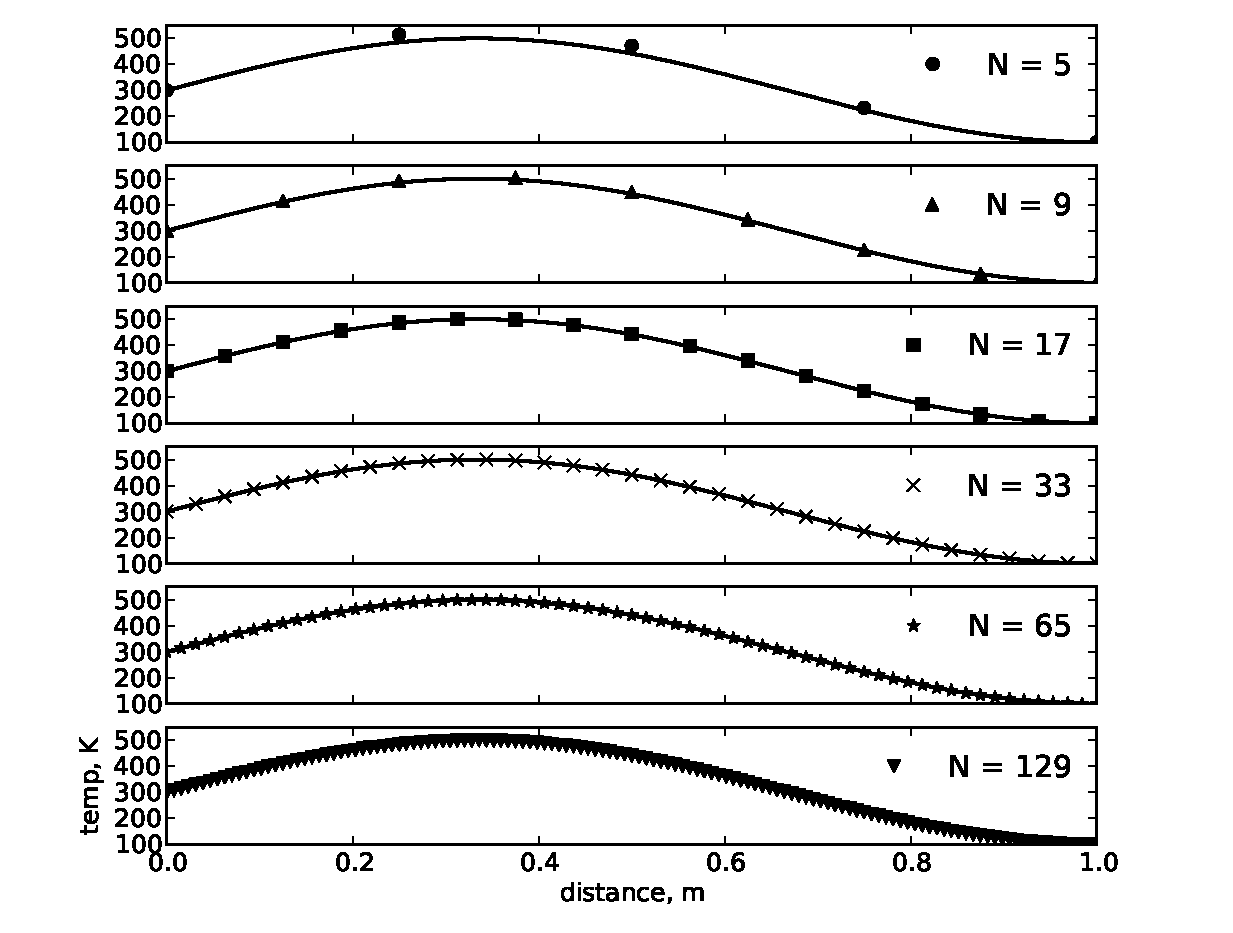
\includegraphics[width=.6\textwidth]{./figs/MMS_profiles.eps}
	\caption{Temperature solution with exact solution overlaid.}
	\label{fig:MMS_profile}
\end{figure}

The relative iterative residuals for the different node numbers and order
of accuracy calculations are shown in \fig{fig:MMS_resid} and \fig{fig:MMS_ooa},
respectively.  The finer grids should have been run longer to reach a lower
iterative error, but the solution is still close.  The observed order of accuracy,
$\hat{p}$, is two when calculated using $L_2$ and 1.5 when using $L_\infty$.  This
method should be second order accurate, and it is.

 
\begin{figure}
	\centering
	\begin{subfigure}[b]{0.475\textwidth}
		\centering
		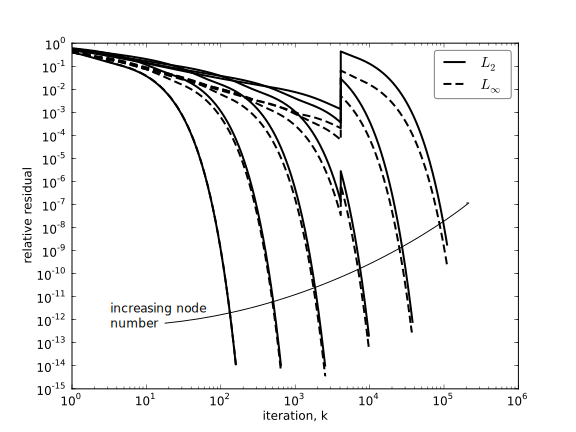
\includegraphics[width=\textwidth]{./figs/MMS_resid.pdf}
		\caption{Residuals}
		\label{fig:MMS_resid}
	\end{subfigure}
	~
	\begin{subfigure}[b]{0.475\textwidth}
		\centering
		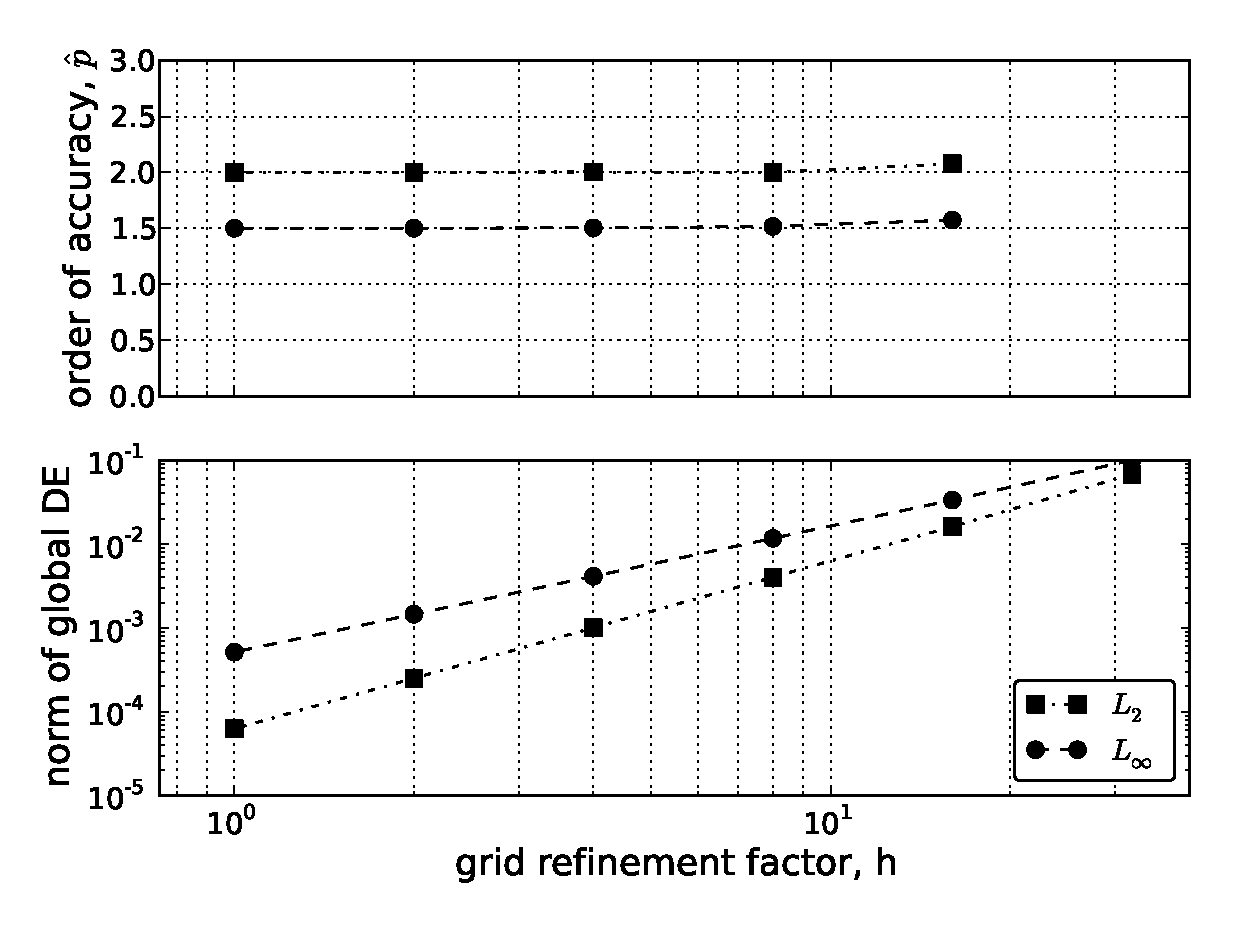
\includegraphics[width=\textwidth]{./figs/MMS_ooa.eps}
		\caption{Order of accuracy}
		\label{fig:MMS_ooa}
	\end{subfigure}
	\caption{Manufactured temperature profiles and iterative residuals.}
\end{figure}

%% -------------------------------------------------------------------------

\section{Part 2}

The goal of part~2 is to solve the 1D unsteady heat equation, like part~1, but
with a different source term and not using the method of manufactured solutions.
The source term is
%
\begin{equation}
	\label{p2_fx}
	f(x) = 100 \left[ 0.25 \left( 0.75 - \left| x - \frac{2}{3} \right| \right) \right] ^ 4 
	\mbox{ K/s}.
\end{equation}
%
The bar is initially at a uniform temperature of \SI{300}{K}, with a constant temperature
boundary condition of \SI{300}{K} at $x=0$ and a temperature derivative of \SI{-200}{K/m}
at $x=1$.  This problem was solved with local time stepping to the steady-state solution,
like in part~1, except that first- and second-order explicit schemes were used
to determine the temperature at the right boundary (and compare how both
perform).  The temperature at $T_{i-1}^n$ and
$T_{i-2}^n$ were expanded in a Taylor series about the end wall point as follows:
%
\begin{align}	
	T_{i-1}^n &= T_i^n + \frac{\p T}{\p x}\bigg|_{i}^n (-\Delta x) + 
				\frac{\p^2 T}{\p^2 x}\bigg|_{i}^n \frac{(-\Delta x)^2}{2} + 
				\mathcal{O}(\Delta x^3) \label{eqn:O1} \\
	T_{i-2}^n &= T_i^n + \frac{\p T}{\p x}\bigg|_{i}^n (-2\Delta x) + 
				\frac{\p^2 T}{\p^2 x}\bigg|_{i}^n \frac{(-2\Delta x)^2}{2} +
				\mathcal{O}(\Delta x^3) \label{eqn:O2}.
\end{align}
%
For the first-order accurate scheme, eq.~(7) is rearranged for $T_i^n$ as
%
\begin{equation}
	T_{i}^n = T_{i-1}^n + \frac{\p T}{\p x}\bigg|_{i}^n + \mathcal{O}(\Delta x^2).
\end{equation}
%
For the second order accurate scheme, we combine eqns.~(7) and (8) such that the
second-terms cancel.  We subtract 4(8) from (7) and rearrange to get
%
\begin{equation}
	T_i^n = \frac{1}{3} \left[ 4 T_{i-1}^n - T_{i-2}^n + 
	2\Delta x \frac{\p T}{\p x}\bigg|_{i}^n \right] + \mathcal{O}(\Delta x^3).
\end{equation}
%
The above equations were used to solve for the temperature at the boundary after all of
the interior nodes had been solved for.

Additionally, for part~2, the Grid Convergence Index (GCI) was used to estimate
the numerical uncertainty in the steady-state solution.  The GCI is define as
%
\begin{equation}
	\label{eqn:gci}
	GCI = \frac{F_s}{r^p - 1} \left| \frac{f_2 - f_1}{f_1} \right|,
\end{equation}
%
where $F_s$ is a factor of safety (3 was used for this study), $r$ is the refinement
factor from going from the coarse (subscript 2) to fine (subscript 1) grids, $p$ is
the order of accuracy of the numerical scheme, and $f$ is the numerical solution at
the different node locations for the different grids.  Note that this assumes one
is in the asymptotic regime, which can be checked by observing the iterative
residual plot.

%% -----

\subsection{Results}

The temperature profiles for using both the first- and second-order is shown
in \fig{fig:p2_profiles}.  The second order accurate scheme converges to the
correct value sooner with a smaller grid than the first order accurate method, which
is expected.  Additionally, the first order method under-predicts the temperature
profile, while the second-order scheme over-predicts.

\begin{figure}
	\centering
	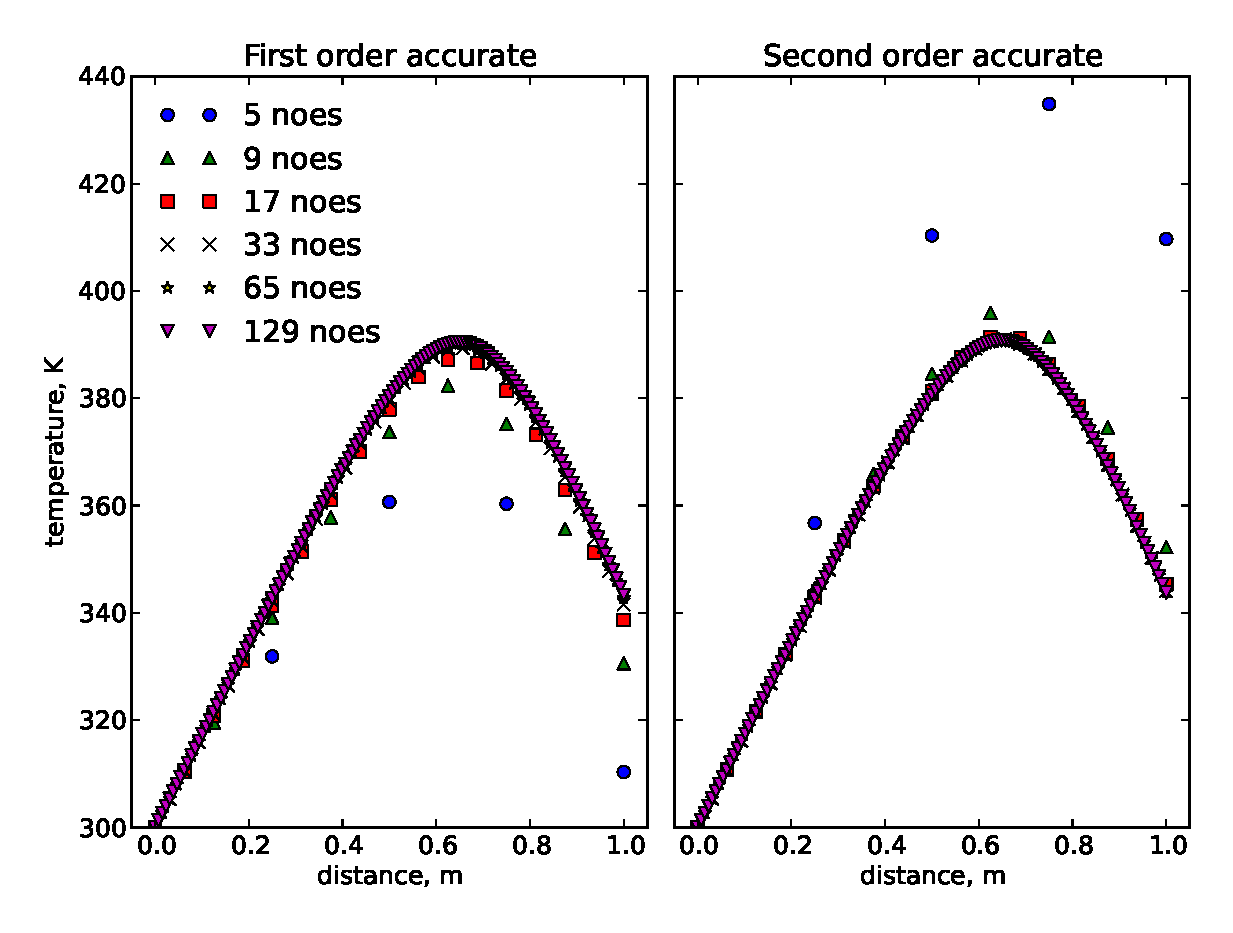
\includegraphics[width=4.5in]{./figs/p2_profiles.eps}
	\caption{Temperature profiles for different meshes and using first and
		second order accurate scheme to find the temperature at $x=1$.}
	\label{fig:p2_profiles}
\end{figure}

The iterative relative residual using both schemes is shown in \fig{fig:p2_relresid}
and the GCI is shown in \fig{fig:p2_gci}.  The fine grid does not reach the 
residual cutoff of \num{1e-12}, but it is close after \num{400000} iterations.
The GCI does a good job of showing the difference between the first- and second- order
accurate schemes.  The finest grid using the first-order method is only slightly
better than the second coarsest grid using the second-order method.

\begin{figure}
	\centering
	\begin{subfigure}[b]{0.475\textwidth}
		\centering
		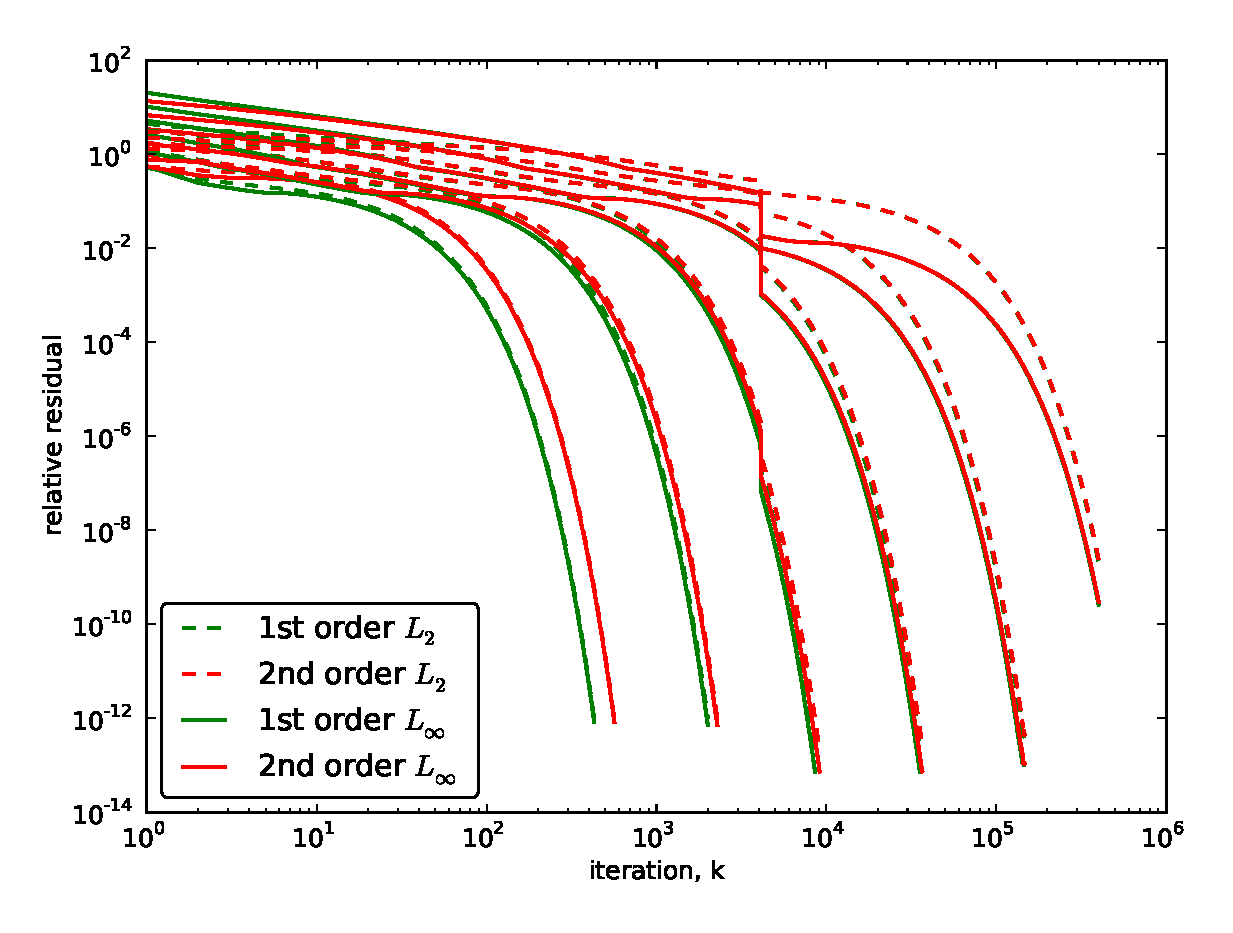
\includegraphics[width=\textwidth]{./figs/p2-relresid.eps}
		\caption{Relative residuals}
		\label{fig:p2_relresid}
	\end{subfigure}
	~
	\begin{subfigure}[b]{0.475\textwidth}
		\centering
		\includegraphics[width=\textwidth]{./figs/p2_gci.eps}
		\caption{Grid convergence index}
		\label{fig:p2_gci}
	\end{subfigure}
	\caption{Temperature solution for first- and second-order accuate scheme.}
\end{figure}

\clearpage
\section{Code and implementation}

The source code for this was written in an IPython notebook, which
is available at \url{https://github.com/isaacyeaton/adv-intro-cfd-2012}.  A pdf
version of this notebook is attached below, but an html version is available
on the Github page as \texttt{hw5.html}.

\includepdf[nup=1x1]{../hw5.pdf}

\end{document}

































